\section{L2 Cache Size Sensitivity}
\label{sec:results:l2size_sensitivity}

\todo{First figure shows how an increasing size of l2 cache causes fewer accesses to l3, and hence all algorithms have fewer request to base their choices on}
\todo{All other figures in general show that when size of private cache increases, the gains of running a custom algorithm over running lru lessens. By this observation it seems that if the choice is either increasing cache space, or utilizing a more advanced algorithm, then the choice may not be obvious.}

In this section, we investigate how increasing the size of private cache available to each processor affects the performance of the algorithms.
We ran the same experiment as in section~\ref{sec:results:base}, but with varying L2 sizes.
The L2 configurations used are shown in table~\ref{}\todo{}, to summarize we utilise cache sizes of 128k, 256k, 512k, and 1024k.
As in previous experiments, we vary the L3 size relative to the workload size.
In this experiment, we only utilize the three random workload groups.
We do this to be able to aggregate and compare 4-core results to 8- and 16-core results.
If results from all 4-core workloads had been used to generate an aggregate, it would have been biased.
This because most of the workloads have specific traits while the random workloads contain benchmarks with mixed traits.

Figure~\ref{fig:results:l2:access} shows the average number of L3 accesses for random workloads with varying L2 cache size.
As can be seen from the graph, by increasing the size of the L2 we are decreasing the number of accesses to the L3 cache.
In other words, the L2 caches are hiding an increasing amount of memory requests from the shared level.
We expect this increased filtering of requests to have an impact on the performance of the implemented algorithms.

Figure~\ref{fig:results:l2:tadip} shows the relative speedup of TADIP compared to LRU measured in STP. 
As seen previously, TADIP performs as good as LRU in both 4- and 8-core workloads with a 128k L2 cache.
With increasing L2 cache size TADIP steadily outperforms LRU with between 0.1\% and 0.6\% depending on the configuration. 
At 16-cores, TADIP underperforms compared to LRU, as previously shown.
We note that, in this case, increasing the L2 size seems to cause a further decrease in TADIP performance, while the opposite is true in the 8-core case.
As covered in section~\ref{}\todo{base} we expect that TADIP suffers in the 16-core workloads because the faction of dueling sets in the cache increases.
We also know that when we increase filtering of memory requests in private levels, TADIP will react slower to changes in application phases, due to its counter architecture.
This last effect does not seem to have a noticeable impact on the results, in the 4- and 8-core runs, but becomes visible in the 16-core runs.

DRRIP as already covered outperforms LRU, figure~\ref{fig:results:l2:drrip} confirms this.
The figure also shows that increasing the L2 size causes a reduction in DRRIP performance.
We know that DRRIP uses a step-wise promotion policy where each successive access causes a block to be promoted by one position.
Naturally less information about success reuse will be available to the shared level as filtering in the private levels increase.
It is consequently not unexpected that DRRIP suffers from increased filtering by private cache levels.
From the figure, we note that DRRIP seems to be slightly less sensitive to small changes in L2 size with increasing core count, but in all cases a 1024k L2 causes DRRIP performance to mimic LRU performance.

In contrast to the previous algorithms, UCP performance increases with L2 cache size in all workloads, as seen in figure~\ref{fig:results:l2:ucp}.
We know that UCP uses a utility algorithm as the mechanism for allocating ways to cores. 
The input to this algorithm changes when we increase filtering of requests to the shared cache level.
As a result, the allocation of ways to cores also is expected to change, but this is the intended mechanism of UCP and should not negatively affect performance.
UCP uses LRU to manage replacement for each core, but UCP under normal circumstances only allows a core to evict one of its own blocks. 
We have already covered that this is why UCP outperforms LRU in the base configuration, in section~\ref{}\todo{base}. 
As filtering increases at the private level, we notice that UCP increases its performance compared to LRU. 
We expect that this is because less information causes LRU to make worse decisions, but this effect is less noticeable in UCP because UCP separates the LRU decisions between cores.

PriSM~\todo{}

Finally figure~\ref{fig:results:l2:pipp} show the performance of PIPP, and figure~\ref{fig:results:l2:pipp-min8} shows the performance of the modified PIPP algorithm.
Since PIPP uses the same utility algorithm as UCP and aims to achieve the same allocations as UCP, we expect them to show similar trends.
This expectation somewhat holds true for the 4-core case, where there is a slight upward trend with increasing L2 size.
However, PIPP underperforms compared to LRU in all workloads, and with increasing core count performance drops significantly.
Why this is happening has already been covered in section~\ref{}\todo{base}.
The modified PIPP algorithm shows a performance development much closer to what is expected, at least for 4- and 8-core workloads.
We observe the same increase in performance with increased L2 cache size as seen in the UCP case. 
However, in the 16-core workloads, the same issues as seen in the PIPP algorithm becomes visible, and performance drops significantly.



\begin{figure}[H]
    \centering
    \begin{subfigure}[b]{0.5\textwidth}
        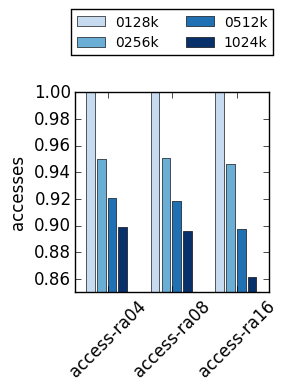
\includegraphics[width=\textwidth]{figures/results/speedup/accesses-accesses-0128k-0100-access}
        \caption{Relative number of accesses to L3 cache with varying L2 size}
        \label{fig:results:l2:access}
    \end{subfigure}
    \begin{subfigure}[b]{0.5\textwidth}
        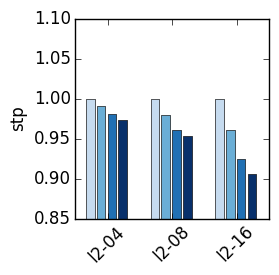
\includegraphics[width=\textwidth]{figures/results/speedup/l2-stp-0128k-tadip-l2}
        \caption{Speedup of TADIP relative to LRU}
        \label{fig:results:l2:tadip}
    \end{subfigure}%
    \begin{subfigure}[b]{0.5\textwidth}
        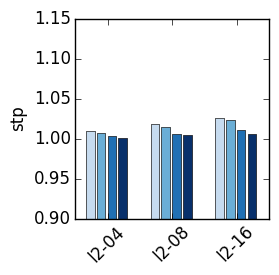
\includegraphics[width=\textwidth]{figures/results/speedup/l2-stp-0128k-drrip-3-l2}
        \caption{Speedup of DRRIP relative to LRU}
        \label{fig:results:l2:drrip}
    \end{subfigure}
\end{figure}
\clearpage
\begin{figure}[H]
    \ContinuedFloat
    \begin{subfigure}[b]{0.5\textwidth}
        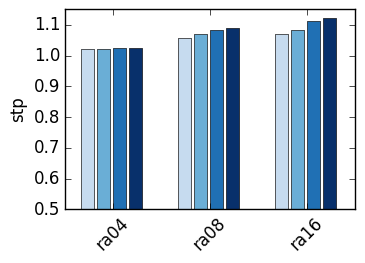
\includegraphics[width=\textwidth]{figures/results/speedup/l2-stp-0128k-ucp-l2}
        \caption{Speedup of UCP relative to LRU}
        \label{fig:results:l2:ucp}
    \end{subfigure}%
    \begin{subfigure}[b]{0.5\textwidth}
        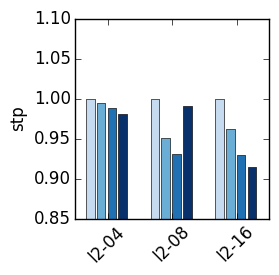
\includegraphics[width=\textwidth]{figures/results/speedup/l2-stp-0128k-prism-l2}
        \caption{Speedup of PriSM relative to LRU}
        \label{fig:results:l2:prism}
    \end{subfigure}
    \begin{subfigure}[b]{0.5\textwidth}
        \includegraphics[width=\textwidth]{figures/results/speedup/l2-stp-0128k-pipp-l2}
        \caption{Speedup of PIPP relative to LRU}
        \label{fig:results:l2:pipp}
    \end{subfigure}%
    \begin{subfigure}[b]{0.5\textwidth}
        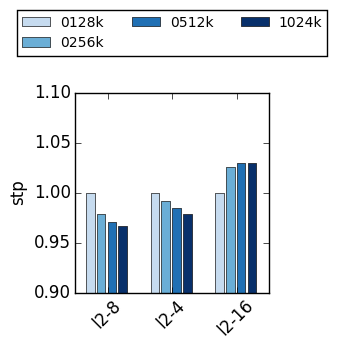
\includegraphics[width=\textwidth]{figures/results/speedup/l2-stp-0128k-pipp-min8-l2}
        \caption{Speedup of PIPP-min8 relative to LRU}
        \label{fig:results:l2:pipp-min8}
    \end{subfigure}
    \caption{Speedup of cache paritition algorithms relative to LRU with increasing private L2 size}
    \label{fig:results:l2}
\end{figure}
